\section{PAC Learnability of Depth Limited Decision Trees [30 points]}
\label{sec:pac-learn-depth}


In this question, you will be showing that depth limited decision trees are PAC
learnable.

Suppose we have a binary classification problem with $n$ Boolean features that
we seek to solve using decision trees of depth $k$. For this question assume trees are complete, meaning each node (other than the leaf nodes) has exactly two children. The figure below shows some
examples of such trees and their depths. 

\begin{tikzpicture}
  \node[draw, circle] (false) at (0,0) {$0$};
  \node[above=0.5cm of false] {Depth = 0};

  \node[draw, circle, right=2cm of false] (true)  {$1$};
  \node[above=0.5cm of true] {Depth = 0};

  \node[draw, rectangle, right=3cm of true] (t21) {$x_1$};
  \node[draw, circle, below=1cm of t21, xshift=-1cm] (t22) {$1$};
  \node[draw, circle, below=1cm of t21, xshift=1cm] (t23) {$0$};
  \draw[->,thick] (t21) -- node[midway, above] {$1$} (t22);
  \draw[->,thick] (t21) -- node[midway, above] {$0$} (t23);  

  \node[above=0.5cm of t21] {Depth=1};

  \node[draw, rectangle, right=4cm of t21] (t31) {$x_1$};
  \node[draw, rectangle, below=1cm of t31, xshift=-1.5cm] (t32) {$x_2$};
  \node[draw, rectangle, below=1cm of t31, xshift=1.5cm] (t33) {$x_3$};
  \node[draw, circle, below=1cm of t32, xshift=-1cm] (t34) {$1$};
  \node[draw, circle, below=1cm of t32, xshift=1cm] (t35) {$0$};
  \node[draw, circle, below=1cm of t33, xshift=-1cm] (t36) {$0$};
  \node[draw, circle, below=1cm of t33, xshift=1cm] (t37) {$1$};

  \draw[->,thick] (t31) -- node[midway, above] {$1$} (t32);
  \draw[->,thick] (t31) -- node[midway, above] {$0$} (t33);

  \draw[->,thick] (t32) -- node[midway, above] {$1$} (t34);
  \draw[->,thick] (t32) -- node[midway, above] {$0$} (t35);
  \draw[->,thick] (t33) -- node[midway, above] {$1$} (t36);
  \draw[->,thick] (t33) -- node[midway, above] {$0$} (t37);    
  \node[above=0.5cm of t31] {Depth=2};  
\end{tikzpicture}

\begin{enumerate}
\item Since decision trees represent a finite hypothesis class, the quantity of
  interest is the number of such trees---i.e., trees with depth $k$ over $n$
  features. Suppose we use $S_n(k)$ to denote the number of the number of trees
  with depth exactly $k$ if we have $n$ features.

  The following questions guide you through this counting process. Recall that
  each answer should be accompanied with an explanation.\emph{If you simply
    write the final answer, you will not get any points.} (\textbf{Please see the note at the end of this questions for further clarification}3).

  \begin{enumerate}
  \item \relax[2 points] What is $S_n(0)$? That is how many trees of depth $0$
    exist?
    
  \item \relax[3 points] What is $S_n(1)$? That is, with $n$ features, how many
    trees of depth $1$ exist?
    
  \item \relax[4 points] Suppose you know the number of trees with depth $i$,
    for some $i$. This quantity would be $S_n(i)$ using our notation. Write down
    a recursive definition for $S_n(i+1)$ in terms of $n$ and $S_n(i)$.

    For this expression, you can assume that we are allowed to the use same
    feature any number of times when the tree is constructed.

  \item \relax[6 points] Recall that the quantity of interest for PAC bounds is
    the $\log$ of the size of the hypothesis class. Using your answer for the
    previous questions, find a closed form expression representing $\log S_n(k)$
    in terms of $n$ and $k$. Since we are not looking for an exact expression,
    but just an order of magnitude, so you can write your answer in the big $O$
    notation.
    
  \end{enumerate}

\item Next, you will use your final answer from the previous question to state a
  sample complexity bound for decision trees of depth $k$.

  \begin{enumerate}
  \item \relax[3 points] With finite hypothesis classes, we saw two Occam's
    razor results. The first one was for the case of a consistent learner and
    the second one was for the agnostic setting. For the situation where we are
    given a dataset and asked to use depth-$k$ decision trees as our hypothesis
    class, which of these two settings is more appropriate? Why?

  \item \relax[4 points] Using your answers from questions so far, write the
    sample complexity bound for the number of examples $m$ needed to guarantee
    that with probability more than $1- \delta$, we will find a depth-$k$
    decision tree whose generalization error is no more than $\epsilon$ away
    from its training error.

  \end{enumerate}

\item \relax[4 points] Is the set of depth-$k$ decision trees PAC learnable? Is
  it efficiently PAC learnable?

\item \relax[4 points] Suppose the number of features we have is large and the
  depth limit we are considering is also large (say, in the thousands or
  more). Will the number of examples we need be small or large? Discuss the
  implications of the sample complexity bound from above.
  
\end{enumerate}

\textbf{NOTE}: In this question we are counting trees that are structurally different instead of functionally different. As an exercise, you can confirm that the following two trees are structurally different but equal in terms of the label they assign to any example, namely the trees are functionally equivalent.


\begin{center}
    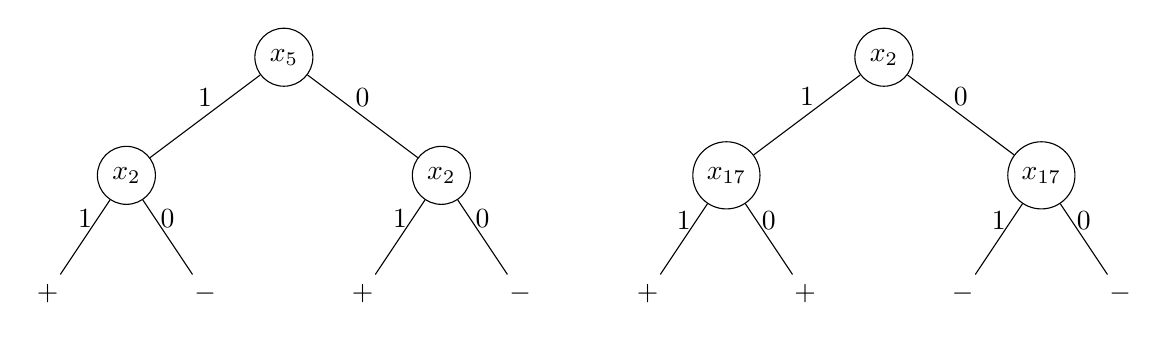
\begin{tikzpicture}[grow = down, level/.style={sibling distance=40mm/#1}, node/.style = {draw, circle}]
    \begin{scope}
      \node[node] {$x_5$} % root
      child { node[node] {$x_2$}
      child { node {$+$}
          edge from parent node [above] {1}}
      child { node {$-$}
          edge from parent node [above] {0}}
        edge from parent node [above] {1}}
      child { node[node] {$x_2$} % x_2
        child { node {$+$}
          edge from parent node [above] {1}}
        child { node {$-$}
          edge from parent node [above] {0}}
        edge from parent node [above] {0}};
    \end{scope}
    \begin{scope}[xshift=3in]
     \node[node] {$x_2$} % root
      child { node[node] {$x_{17}$}
      child { node {$+$}
          edge from parent node [above] {1}}
      child { node {$+$}
          edge from parent node [above] {0}}
        edge from parent node [above] {1}}
      child { node[node] {$x_{17}$} % x_2
        child { node {$-$}
          edge from parent node [above] {1}}
        child { node {$-$}
          edge from parent node [above] {0}}
        edge from parent node [above] {0}};
    \end{scope}
    \end{tikzpicture}
  \end{center}


